\chapter{Design}

For the initial implementation, a single Android app was chosen to test. Despite
this, the library should be generic enough to easily integrate into any Android
application.

There are a few core problems to solve.
One is making the participant use the application in the structured way needed to
gather relevant data. The second is to find a way to enable the developer to integrate
the testing into the application and capture relevant information. The data then needs
to be transported back to the developer, and presented in a way that makes it easy to spot
problem areas in the interface. In addition, the participants need to be encouraged to complete the testing process.

Due to the crowdsourced nature of the system, and the fact that no member of the
development team will be present during the testing, the ``think aloud'' aspect
of traditional testing will be missing. It would, of course, be possible to
record the subject speaking as they navigate the application, but it would not
be feasible to collect and aggregate that data automatically from many
participants. Otherwise, the system will incorporate the same ideas as
traditional usability testing.

\section{User Facing Design}

On starting the testing, the user is shown a screen explaining how the testing
will work. They are then presented with a scenario/task for them to complete. On
completion of the task, they will be either given a successive task, or a screen
thanking them for participating. Since multiple tasks would usually be presented to the user in a normal testing session, the developer is able to group tasks together to be performed successively. They are also able to control whether a task follows on from the previous one, or whether they all begin from a common screen. This will be useful for most tasks, where, for example, the developer wants the user to start from a specific screen such as the home screen of the application.

\subsection{Early Versions and Gamification}

In an attempt to keep the user being tested engaged, and thus increasing the likelihood they would complete more of the testing, a game aspect of the framework was considered. In early
iterations the participant could score points by completing tasks. During a task an overlay would show how long the user is taking (\emph{Figure~\ref{fig:initial-overlay}}) and on completion of the task
they would be assigned a number of points relative to how quickly they did it.
Early evaluation of this prototype highlighted a couple of concerns with this approach. Firstly, showing the user how
long they are taking and encouraging them to complete the task as quickly as
possible could cause the participant to focus on the on screen timer instead of other elements of the interface, resulting in behaviour that did not necessarily match real world usage.
Additionally, the point system did not seem to work as hoped, missing crucial aspects that usually make point systems encouraging.  Since the "game" was not really repeatable, and points were not ranked against any other player or used for any other purpose, participants did not see the point (HA I AM SO FUNNY) in gathering them. 

\begin{figure}[ht!]
  \centering 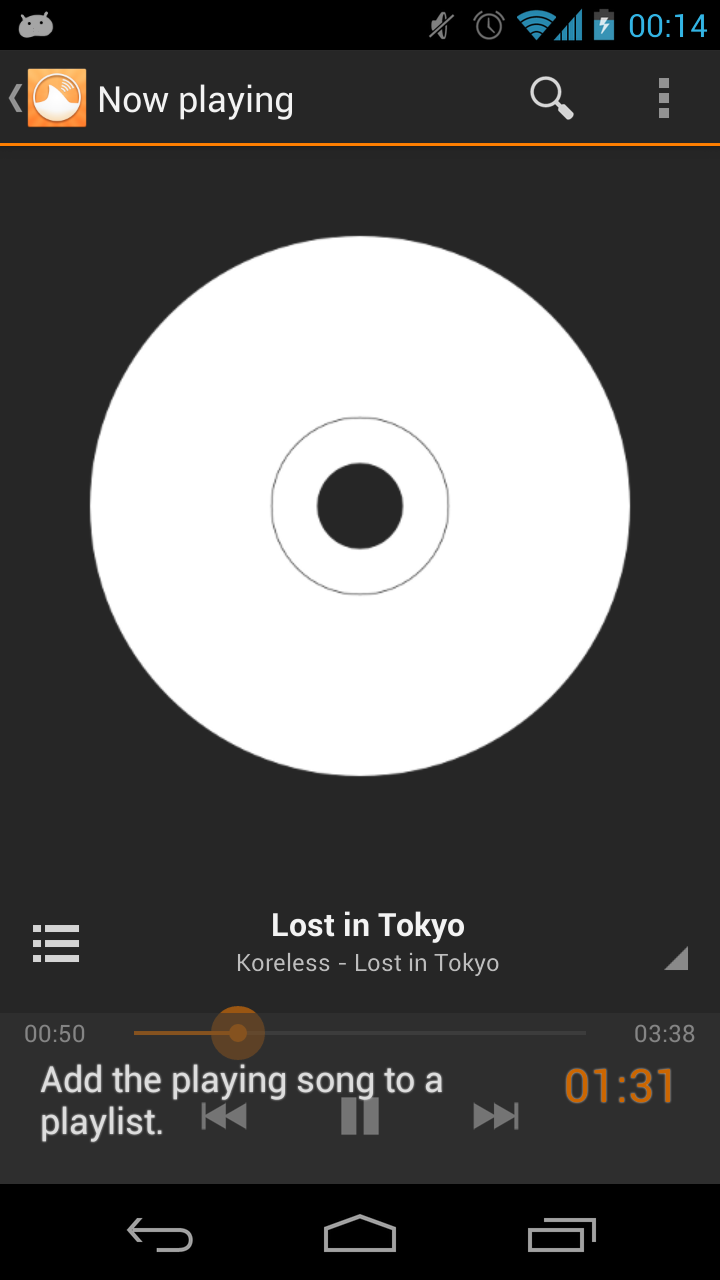
\includegraphics[width=0.5\textwidth]{images/time-taken}
  \caption{The task overlay in early iterations of the project.}
  \label{fig:initial-overlay}
\end{figure}

Due to these issues, this aspect of the software was removed and it no longer encourages
the participant to be competitive. The screen that appears at the beginning of each task now displays
progress that the participant has made through the tasks, hopefully encouraging
the user to complete the process. If the developer wished to provide a reward (such as
unlocking easter eggs or additional features within the app) it would be possible to implement using
the library.

\subsection{In-task UI}

\emph{Figure \ref{fig:initial-overlay}} also shows how the early version of the in-task UI was an overlay over the application interface. While this was semi-transparent, it still had a tendency to obscure important controls, making it harder to use the application. This was refined after the initial evaluation so it no longer obscures content while still displaying important information about the task. The final UI can be seen in \emph{Figure \ref{fig:final-task-overlay}}. While placing an extra piece of interface at the top of the screen affects the height available to the application, android apps must adapt to different screen sizes anyway, and the space taken up is designed to be as small as possible. Using this design also enables controls to be placed in the in-task UI, here used for an "Abandon" button.

\begin{figure}
  \centering
  \missingfigure{Show the new in-task UI}
  \label{fig:final-task-overlay}
\end{figure}

\subsection{Abandoning Tasks}

It's likely that for some tasks, a participant might get stuck, and not be able
to complete it. In these cases it seems unfair to penalise them, since the
interface could be too unintuitive or confusing. Worse, this is usually the case
where the developer could benefit most from the feedback, and if the participant
were penalised it could discourage them from continuing with the testing. To
combat this, as part of the overlay that appears while performing a task a
button allows the participant to abandon the current task at any point. This allows the participant to easily continue the testing, and if many people abandon the same task provides a quick indication of tasks that may be especially difficult to complete.

\section{Developer feedback}
\label{sec:developer-feedback}

To be an effective form of feedback, the system also needs a way for the developer to view the data gathered and identify issues.

There are a few important considerations that were made when designing this:

\begin{itemize}
  \item The developer should be able to see as much of the data gathered as possible.
  \item The aggregate performances of many users are far more important than the performance of individual users.
  \item Problem areas within a task should be easy to spot.
  \item Even bigger issues such as tasks that are commonly abandoned should be easy to spot.
\end{itemize}

Some of these criteria are satisfied easily, for example by highlighting tasks with a success rate lower than a certain percentage, but others are harder.

Depending on the data gathered there are a large number of ways of presenting the results to the developer. In this project, a simple interface was developed which hopes to satisfy the criteria above.

\subsection{Capturing Navigation}

Each ``run'' through a task can be represented as a sequence of navigation points. Each screen of
an Android app is made up of Activities, or Fragments within an Activity. These provide a starting
point, and each new Activity is automatically added as a new navigation point. In addition, 
the developer can choose to include Fragment changes, and any other event that they deem important to 
the navigation. Extra data can be passed along with the navigation point. This is useful in situations
where the same screen might be used to display different sets of data, for example on a search screen the
developer might want to include the search query used. A simple navigation path is shown in Figure \ref{fig:task-navigation}

\begin{figure}
 \centering
 \missingfigure{Mockup of a simple task navigation path.}
 \label{fig:task-navigation}
\end{figure}

Once the navigation path data has been captured from a number of participants' run throughs of a
task, the paths are merged to give a navigation graph, as shown in Figure \ref{fig:task-navigation-tree}. Each path from one node to the next shows the percentage of participants who took that path, and the most
common paths from the start screen to either completing or abandoning the task can be seen.

\begin{figure}
 \centering
 \missingfigure{Mockup of some merged navigation paths.}
 \label{fig:task-navigation-tree}
\end{figure}

An issue with this approach immediately showed during early evaluation of the system. When participants were unsure of how to proceed, they would often try many different options, quickly abandoning them and returning to the previous screen when it became clear the action they took was not the correct one.
After a few users doing this the navigation tree became particularly messy and unreadable 
(Figure \ref{fig:task-navigation-mess}).

\begin{figure}
 \centering
 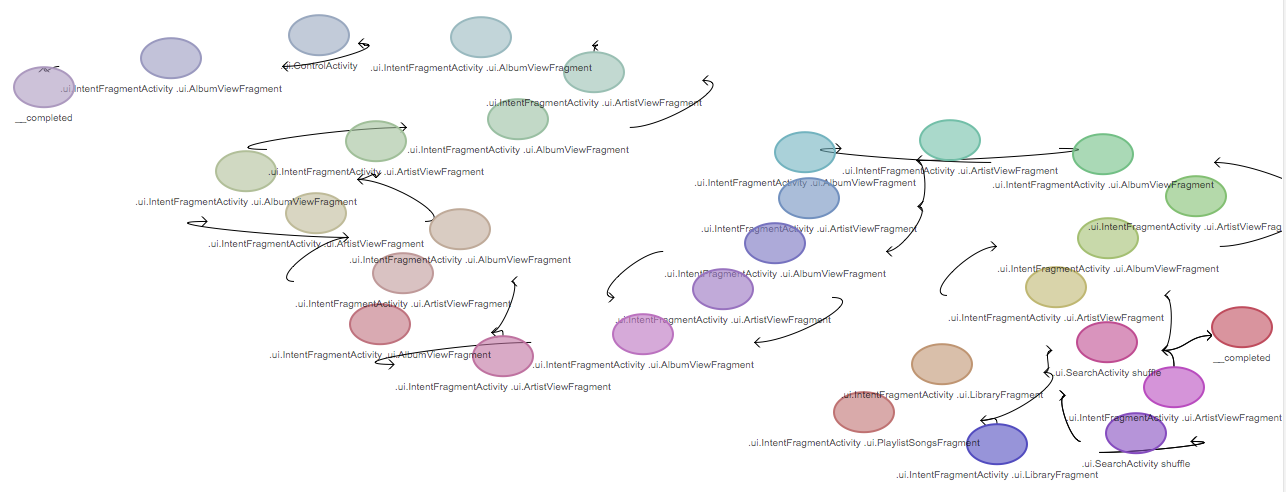
\includegraphics[width=\textwidth]{images/messy-graph}
 \caption{Messy graphs produced when when participants backtrack.}
 \label{fig:task-navigation-mess}
\end{figure}

A simple fix for this was to not include part of the path in the graph when the user immediately returns
to the previous point (Figure \ref{fig:task-navigation-mess-fixed}). Since this information is still important to indicate usability problems, the average number of these ``backtracks'', if any, is shown below each node in the graph.

\begin{figure}
 \centering
 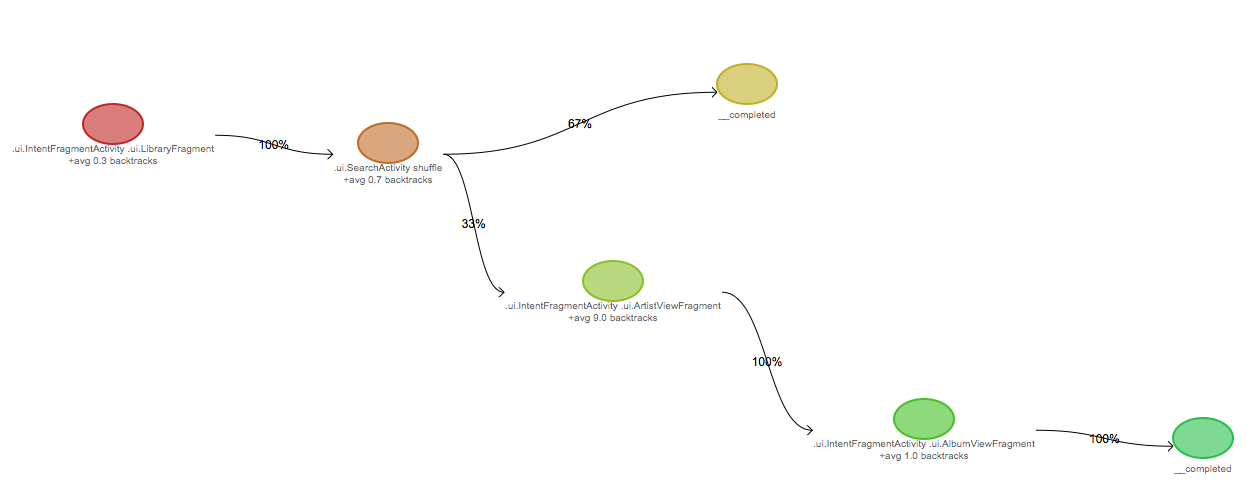
\includegraphics[width=\textwidth]{images/fixed-graph}
 \caption{The same graph after filtering backtracking.}
 \label{fig:task-navigation-mess-fixed}
\end{figure}